\documentclass{article}

\usepackage[pdftex]{graphicx}
\usepackage{siunitx}

% *** CITATION PACKAGES ***
%
\usepackage{cite}
% cite.sty was written by Donald Arseneau
% V1.6 and later of IEEEtran pre-defines the format of the cite.sty package
% \cite{} output to follow that of the IEEE. Loading the cite package will
% result in citation numbers being automatically sorted and properly
% "compressed/ranged". e.g., [1], [9], [2], [7], [5], [6] without using
% cite.sty will become [1], [2], [5]--[7], [9] using cite.sty. cite.sty's
% \cite will automatically add leading space, if needed. Use cite.sty's
% noadjust option (cite.sty V3.8 and later) if you want to turn this off
% such as if a citation ever needs to be enclosed in parenthesis.
% cite.sty is already installed on most LaTeX systems. Be sure and use
% version 5.0 (2009-03-20) and later if using hyperref.sty.
% The latest version can be obtained at:
% http://www.ctan.org/pkg/cite
% The documentation is contained in the cite.sty file itself.



% *** MATH PACKAGES ***
%
\usepackage{amsmath}
% A popular package from the American Mathematical Society that provides
% many useful and powerful commands for dealing with mathematics.
%
% Note that the amsmath package sets \interdisplaylinepenalty to 10000
% thus preventing page breaks from occurring within multiline equations. Use:
\interdisplaylinepenalty=2500
% after loading amsmath to restore such page breaks as IEEEtran.cls normally
% does. amsmath.sty is already installed on most LaTeX systems. The latest
% version and documentation can be obtained at:
% http://www.ctan.org/pkg/amsmath



% correct bad hyphenation here
\hyphenation{op-tical net-works semi-conduc-tor}

%\usepackage[utf8]{inputenc}
%\usepackage{helvet}
%\usepackage[usenames,dvipsnames,svgnames,table]{xcolor}
%\usepackage{graphicx}
%\usepackage{caption}
%\usepackage{subcaption}
%\usepackage{url}
%\usepackage{amstext}

%\bibliographystyle{IEEEtran}

% Title Page
\title{Mapping Deforestation with Recurrence Metrics of Sentinel-1 time series}
\author{Felix Cremer, Mikhail Urbazaev, Christiane Schmullius and Christian Thiel}

%\IEEEauthorblockA{Chair of Earth Observation, Friedrich-Schiller University, Jena,Germany\\
%Email: felix.cremer@uni-jena.de}

\begin{document}
\maketitle
%\tableofcontents
\begin{abstract}
  Forest ecosystems
  REDD+ process
  order of time series
  SAR

%Keywords:Recurrence, SAR, time series, remote sensing
%
\end{abstract}
\section{Introduction}
The tropical forest ecosystems stabilise the world climate\cite{}, the protection of the biodiversity \cite{} and
for the well being of a vast amount of the global popu-
lation\cite{}.
 In the last decade remote sensing technologies have
played a substantial role in the consistent, reliable and timely
information gathering about forest cover changes. With the
REDD+ mechanism the use of remote sensing to monitor
and map deforestation and degradation processes increased.
Forest/Non-Forest maps are mostly operationally if
they are based on optical sensors. Especially in the tropics,
the optical imaging is hindered by clouds. In this study we
 propose a deforestation mapping approach based on SAR time
series.

Misses overview about established methods.
Especially the percentile range

\section{Method}

\subsection{Recurrence Plots}

Recurrence plots (RP) have been proposed by Eckmann et al 1987. They are a method to visualize the recurrences of a time series.
They are defined as follows:
$$R_{i,j} = \theta(\epsilon - \lvert x_i - x_j \rvert), i,j = 1,...,N$$
hereby $\epsilon$ is a threshold value which indicates up to which distance two time steps are viewed as similar.
$\theta$ is the Heaviside function which sets everything below zero to zero and every positive value to one.
N is the number of time steps.
This leads to a quadratic matrix with black dots where the time steps are similar to each other and white dots where they are distinct.
The main diagonal is always black, because every time step is similar to itself.
It is a nonlinear data analysis tool.
Figure \ref{rplots} shows example Recurrence plots of a sum of two sine waves with different frequencies,
a step function from three to zero with an overlaid white noise with standard deviation 1 and third a sine wave with overlaying trend.
For the composition of two different frequencies we can see a regular pattern with distinguished diagonals which are indicating the frequency.
In the noisy step function we see four distinct quadrants in the recurence plot.
In the two quadrants near the main diagonal every point is randomly similar to other points in this part of the time series with a high probability.
In the other two quadrants, the probability is low, that two points are similar to a point in the other part of the step function.
In the third example, we see a clear pattern, but these patterns are fading out to the edge of the recurrence plot.
This is due to the difference of the values at the beginning and the end of the time series.
Therefore we can use this pattern as an indicator for a trend in the time series.

\begin{figure}
  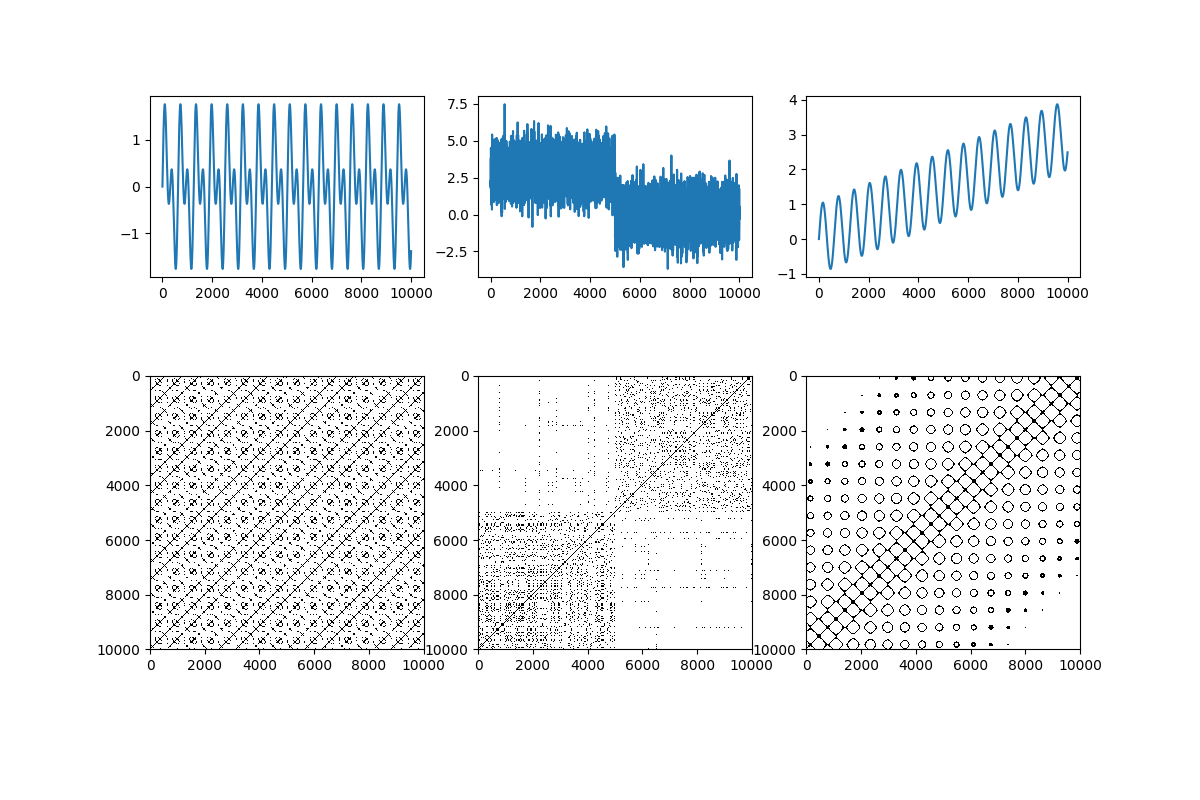
\includegraphics[width=\textwidth]{figs/rp_methods.png}
  \caption{Recurrence Plots for a sine wave, a step function with noise, and a sine wave with trend.}
  \label{rplots}
\end{figure}

These visual patterns can be quantified using recurrence quantification analysis (RQA)\cite{Zbilut}.
The simplest measure is the recurrence rate (RR) which is the number of recurrences in a recurrence plot devided by the squared number of time steps.
It measures the density of the recurrence points in a RP.
Another measure is the trend.
It is defined as
$$ TREND= \frac{\sum_{\tau=1}^{\tilde{N}}(\tau - \tilde{N}/2)(RR_\tau - \langle RR_\tau \rangle)}{\sum_{\tau=1}^{\tilde{N}}(\tau - \tilde{N}/2)}.$$
It is a linear regression coefficient over the recurrence rate of the diagonals in comparison to their distance to the main diagonal.
It indicates if the process is drifting.
For an overview of RQA measures see  \ref{RQA_table} and for an in depth discussion \cite{Marwan06}.
All of the results have been produced using the Julia RecurrenceAnalysis.jl package\cite{RQA.jl}.


\section{Experimental Results}
\subsection{Data and Preprocessing}
We test the separability of stable forest and deforestation on two testsites in Mexico.
One is mostly covered by temperate forests in central Mexico,
the other is situated on the Yucatan peninsula and is covered by tropical dry forests.
Figure \ref{testsites} show very high resolution Pléiades data of the two testsites.

\begin{figure}
  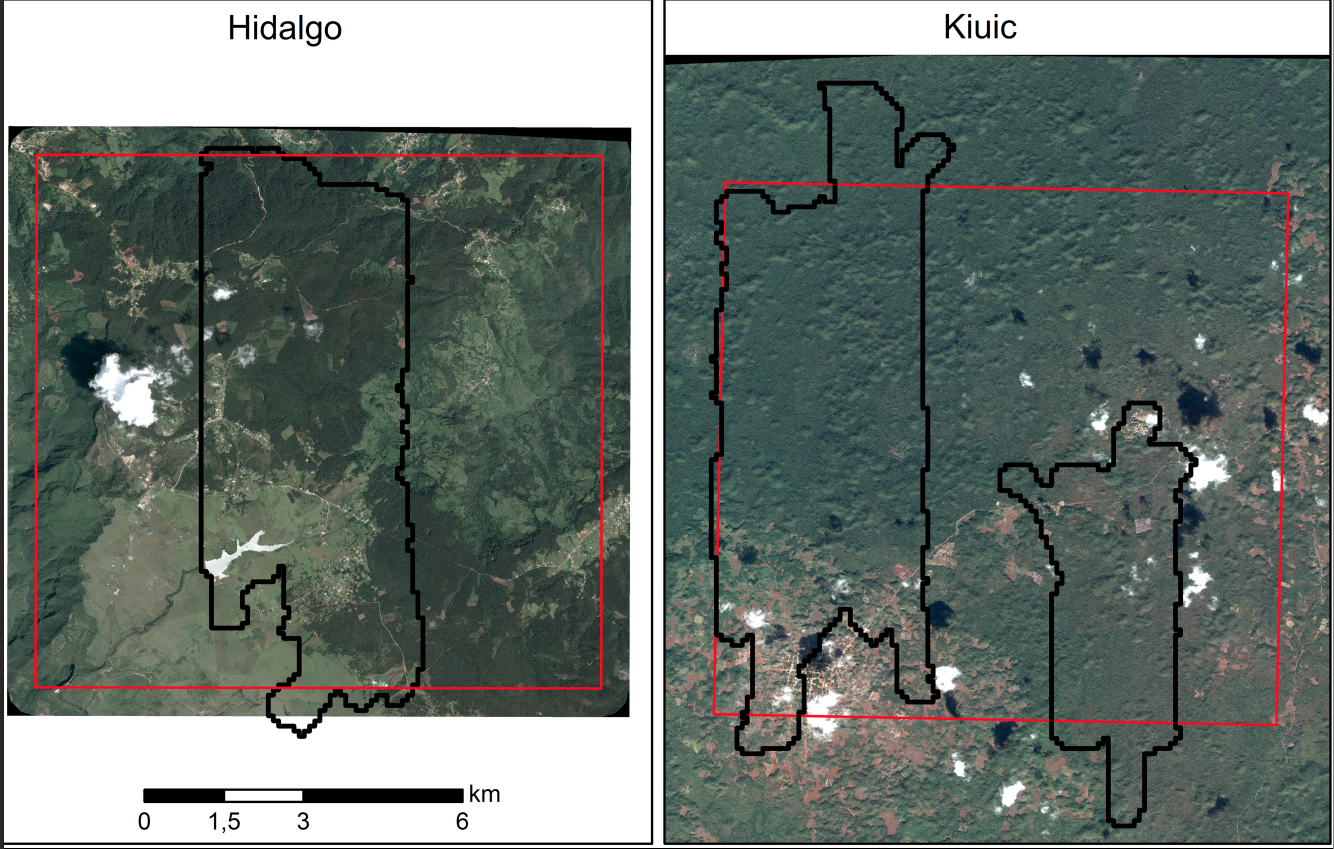
\includegraphics[width=\textwidth]{figs/SEN4REDD_testsites.png}
  \caption{The testsites are located in Mexico and are dominated by temperate forests (Hidalgo) and tropical dry forest(Kiuic).}
  \label{testsites}
\end{figure}

The data have been preprocessed using the SNAP software \cite{SNAP} in version 6.
The single time steps are multilooked to a \SI{10}{\m} x \SI{10}{\m} pixel spacing.
The orthorectification is based on the original orbit state vectors and the \SI{30}{\m} SRTM digital elevation model\cite{SRTM}.
The preprocessing also included radiometric terrain flattening after \cite{Small} which results in $\gamma^0$ backscatter values.
All images were coregistered in the DEM geometry after geocoding to achieve a subpixel coregistration precision which is of eminent importance when the pixels are investigated in the temporal domain only.




\subsection{Separability analysis}

Figure \ref{rpforest} shows the recurrence plots of a neighbourhood of examplary forest and deforestation areas.
The upper figures shows the time series of a 7x7 matrix of a deforested area (left) and a stable forest (right) with the mean of these pixels in red respectively green.
The bottom figures show the grayscale of the corresponding recurrence plots.
Black points are similar in every pixel of the neighborhood and white points in none.


\begin{figure}
  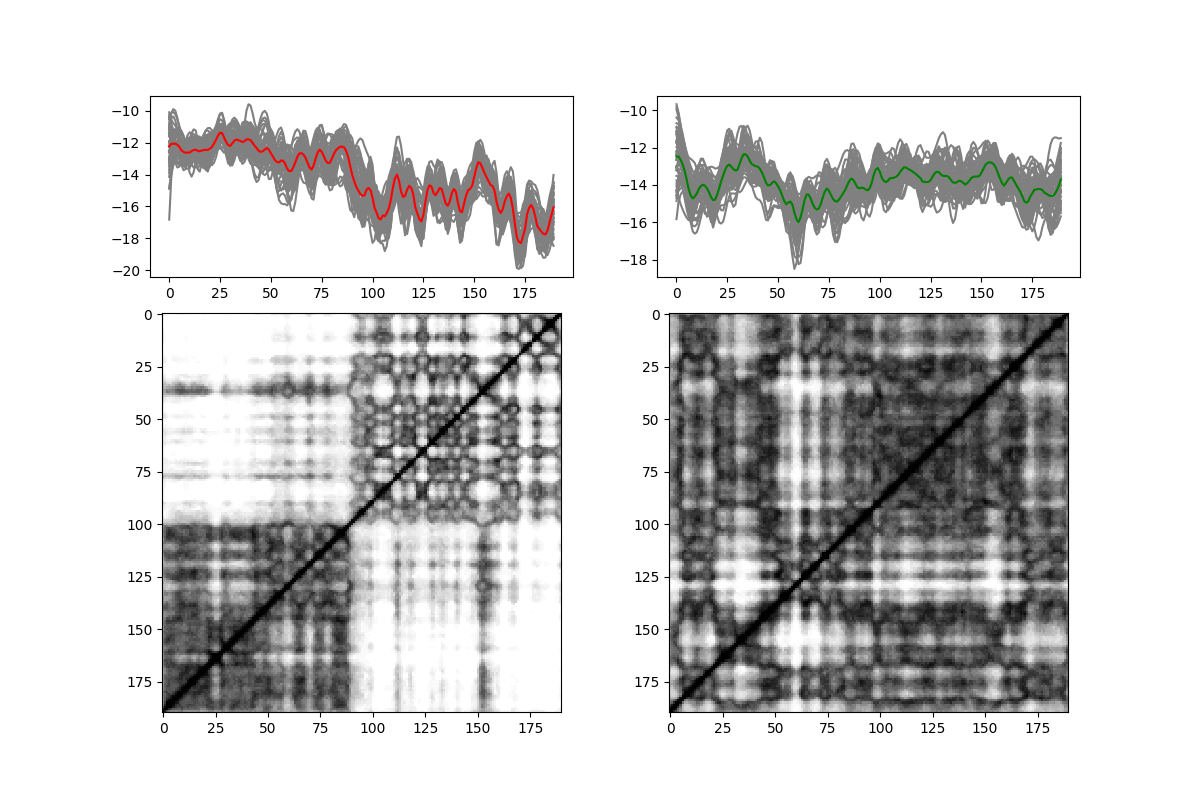
\includegraphics[width=\textwidth]{figs/S1_Hidalgo_timestack_20km_VH___lin_20_test_tandemdem12_emd__rp_deffor_3.png}
  \caption{Recurrence Plots for a 3x3 matrix of deforestated(left) and stable forest(right) pixels.
           The gray lines in the above figure are all pixels and the colored line is the mean of these pixels.}
  \label{rpforest}
\end{figure}

Figure \ref{trend} shows the RQA TREND statistic from two year VH data from march 2017 till march 2019.
For this time frame are 187 time steps available.
The red polygons are deforestations which happened between october 2017 and july 2018 and the green are stable forest areas.
Most of the deforested areas are clearly distinguishable as a distinct black area compared to the surrounding grey.
The not detected deforestation areas are too late in the sensing period.
So that the backscatter change due to the deforestation did not have a long enough effect on the TREND statistic.



\begin{figure}
  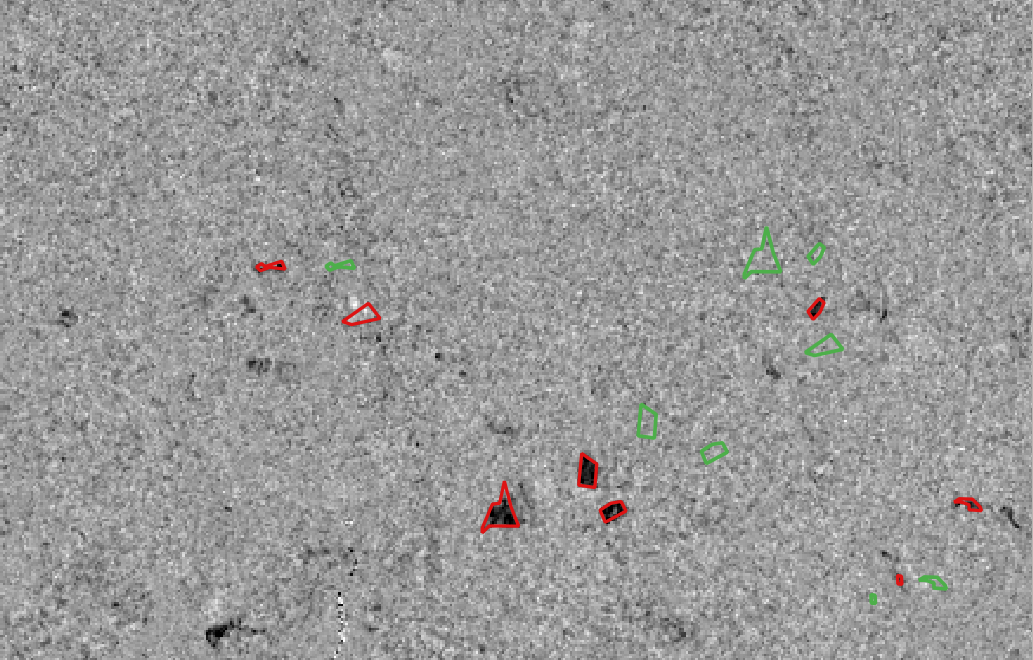
\includegraphics[width=\textwidth]{figs/TREND_Hidalgo_2016.png}
  \caption{RQA TREND statistic.  The red polygons are deforestations between October 2017 and July 2018 and the green polygons are stable forest areas.
  These polygons have been select from VHR Pleiades data.}
  \label{trend}
\end{figure}


Figure \ref{hist} shows the histograms for the RQA trend metric and the percentile range for the deforestation areas in red and the stable forest areas in green.

Show that the TREND metric is enhancing the separability of deforested areas and stable forests.
Quantify it.


Is there a recommendation, which threshold we should use for the percentile range?

\section{Discussion}

Do I need to do a comparison against optical deforestation maps?
Will do a comparison against the percentile range.

Should I show the deforested area in the testsite figure?
Yes please. If I am showing the testsite figure at all.
\section{Summary and Conclusion}
In this paper we showed, that the use of the inherent order of a time series conveys information,
which can be used to better map deforestation.



\section*{Acknowledgment}
This work was funded by the DLR in the Sentinel4REDD project (FKZ:50EE1540) and
the DFG project HyperSense.
This work uses Copernicus Sentinel data 2017-2019.



\bibliography{literatur}

\end{document}
